\documentclass[a4paper]{article}

\usepackage{Sweave} %--------------------------------!
\usepackage{amsmath}
\usepackage{amssymb}
\usepackage{amsthm}
\usepackage{fancyhdr}
\usepackage[usenames, dvipsnames]{color}
\usepackage{verbatim}

\oddsidemargin 0cm
\topmargin -2.4cm     %I recommend adding these three lines to increase the
\textwidth 16.5cm   %amount of usable space on the page (and save trees)
\textheight 27.5cm

\newcommand{\question}[2] {\vspace{.25in} \hrule\vspace{0.5em}
\noindent{\bf #1: #2} \vspace{0.5em}
\hrule \vspace{.10in}}
\renewcommand{\part}[1] {\vspace{.10in} {\bf (#1)}}

\newcommand{\myname}{Xuan Han}
\newcommand{\myhusky}{han.xua@husky.neu}
\newcommand{\myhwnum}{9}

\setlength{\parindent}{0pt}
\setlength{\parskip}{5pt plus 1pt}

\pagestyle{fancyplain}
\lhead{\fancyplain{}{\textbf{HW\myhwnum}}}      % Note the different brackets!
\rhead{\fancyplain{}{\myname\\ \myhusky}}
\chead{\fancyplain{}{1 2}}


\begin{document}
\Sconcordance{concordance:graph.tex:graph.Rnw:%
1 43 1 1 2 1 0 3 1 3 0 1 2 3 1 1 2 1 0 6 1 4 0 1 2 2 1 1 2 1 0 1 15 13 %
0 1 2 1 1 2 2 1 1 4 0 1 2 2 1 1 2 1 0 1 1 4 0 1 2 2 1 1 2 1 0 1 1 30 0 %
1 2 4 1 1 5 8 0 1 2 8 1 1 2 1 0 2 1 1 7 6 0 1 1 5 0 1 1 5 0 4 1 4 0 1 2 %
1 1 1 8 7 0 1 1 5 0 1 1 5 0 4 1 4 0 1 2 8 1}


\title{Data Mining Assignment \myhwnum}
\author{\myname \\
        \myhusky}
\date{\today}
\maketitle

\thispagestyle{plain}

\begin{Schunk}
\begin{Sinput}
> library(igraph)
> edge.table <- read.table("yeast_broad.tsv", header = FALSE, stringsAsFactors = F)
> load("yeast_names.Rdata")
> G <- graph.data.frame(edge.table, vertices = vertex.table, directed = TRUE)
\end{Sinput}
\end{Schunk}


\question{1}{Yeast}
\part{a}{Degree BC PR}
\begin{Schunk}
\begin{Sinput}
> G.degree = degree(G)
> G.bc = betweenness(G)
> G.pr = page.rank(G)$vector
> par(mfrow = c(2,2))
> hist(log(G.degree))
> hist(log(G.bc))
> hist(log(G.pr))
\end{Sinput}
\end{Schunk}
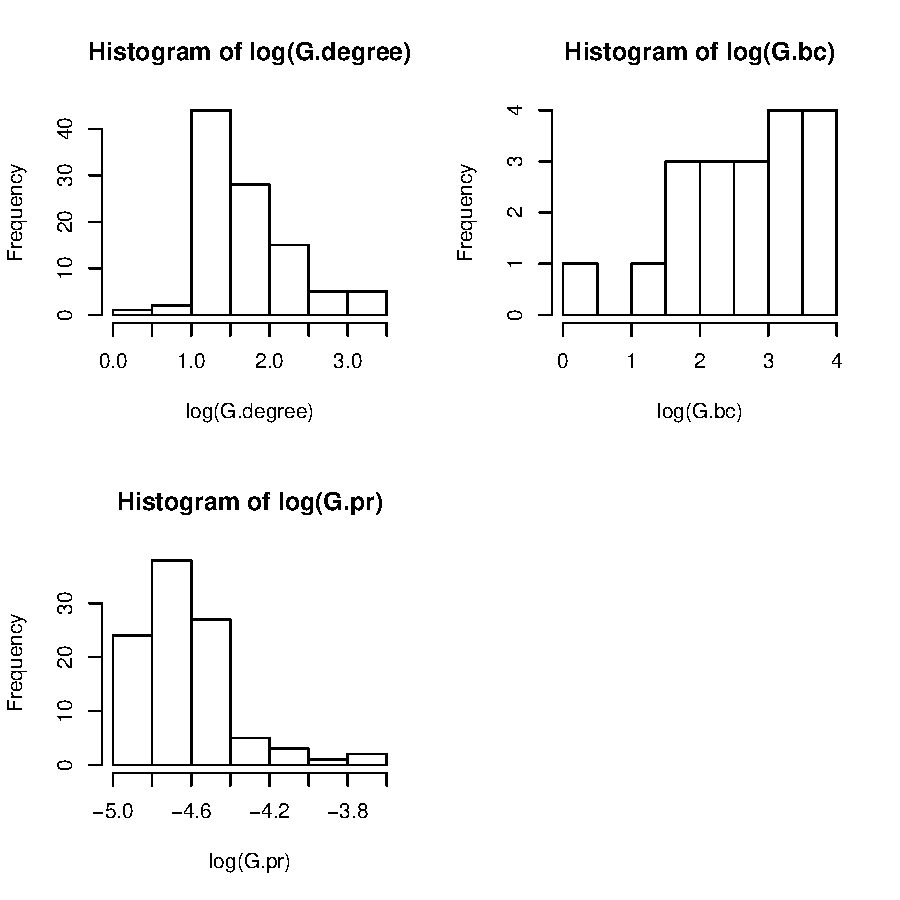
\includegraphics{graph-1a}

\newpage
\part{b}{HITS}
\begin{Schunk}
\begin{Sinput}
> m = as.matrix(get.adjacency(G))
> hits = function(A, round){
+     hub = rep(1, dim(A)[1])
+     auth = rep(1, dim(A)[1])
+ 
+     while(round > 0) {
+         auth = t(A) %*% hub
+         auth = auth / sqrt(sum(auth ^ 2))
+         hub = A %*% auth
+         hub = hub / sqrt(sum(hub ^ 2))
+         round = round - 1
+     }
+     result <- list(hub=hub,auth=auth)
+     return(result)
+ }
> G.hub = hits(m, 20)$hub
> G.auth = hits(m, 20)$auth
> par(mfrow = c(2, 1))
> hist(log(G.hub))
> hist(log(G.auth))
\end{Sinput}
\end{Schunk}
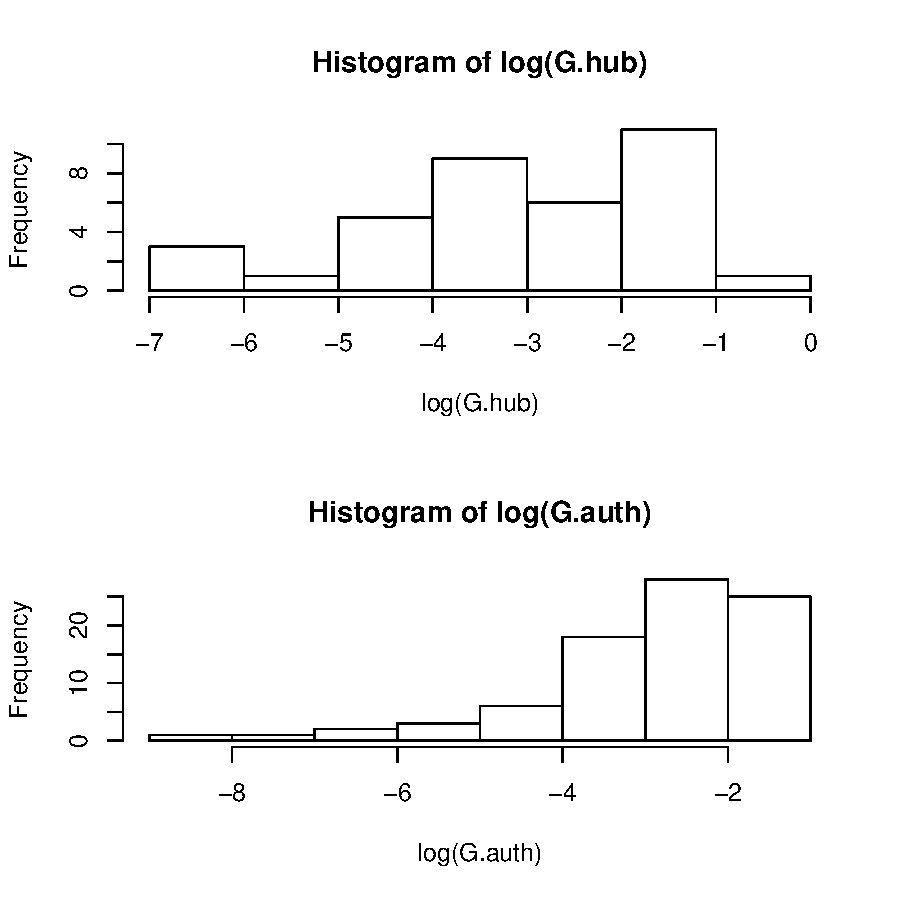
\includegraphics{graph-1b}

\newpage
\part{c}{Compare}
\begin{Schunk}
\begin{Sinput}
> feature = data.frame(degree = G.degree, bc = G.bc, pr = G.pr, hub = G.hub, auth = G.auth)
> pairs(feature)
\end{Sinput}
\end{Schunk}
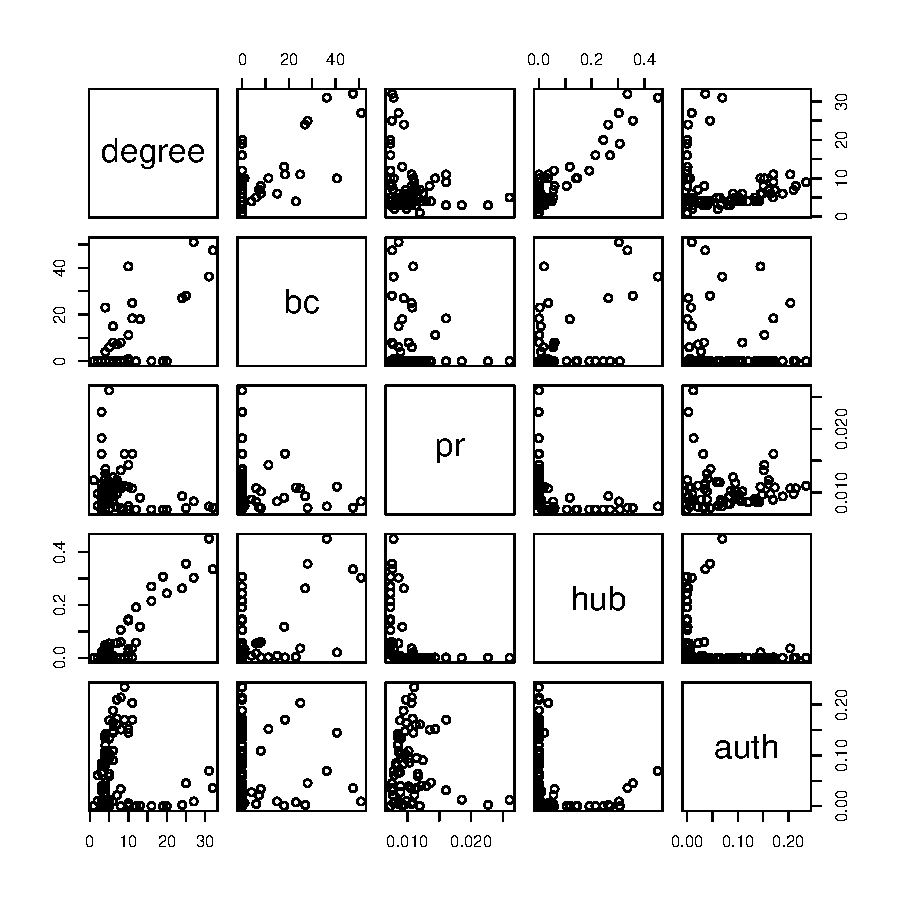
\includegraphics{graph-1c}

% YOL067C

\begin{Schunk}
\begin{Sinput}
> gap = abs(rank(G.auth) - rank(G.degree))
> rank(gap)
\end{Sinput}
\begin{Soutput}
 YCL066W  YCL067C  YCR040W  YCR096C  YCR097W  YDR081C  YDR421W  YDR463W 
     1.5      3.0     11.0     16.0     71.5      9.0     49.5     94.0 
 YFL021W  YGL035C  YGL209W  YGL254W  YGR044C  YHR006W  YIR017C  YJL056C 
    87.0     88.0     95.5      4.5     21.0     57.0     59.0     95.5 
 YJL089W  YJL110C  YJR147W  YKL020C  YKR034W  YLR013W  YLR098C  YML051W 
    91.0     79.0     49.5     92.5     86.0     99.0     92.5     35.0 
 YML099C  YML113W  YMR019W  YMR042W  YMR280C  YNL103W  YOL067C  YOL089C 
    73.0     97.5      6.5     49.5     67.0      9.0    100.0     97.5 
 YOR032C  YPL038W  YPL248C  YPR199C  YKL178C  YPL187W  YDR103W  YCR039C 
    82.0     82.0     90.0     89.0     49.5     14.5     14.5     22.5 
 YDR042C  YDR317W  YCL065W YIL002WA YCR018CA  YCR019W  YDR078C  YDR079W 
    12.5      9.0     30.0     22.5     25.5     25.5     65.5     65.5 
 YDR084C  YGL001C  YGR071C  YGR072W  YHR156C  YHR157W  YJL085W  YJR011C 
    34.0     39.0     32.5     32.5     63.5     63.5     68.5     31.0 
 YLR261C  YLR262C  YMR228W  YNR049C  YOL126C  YOL159C  YDR040C YDR210WD 
    82.0     82.0     82.0     47.0     52.0     58.0     24.0      4.5 
 YDR520C  YDR522C  YGR271W  YLR023C  YMR098C  YMR258C  YBR019C  YBR020W 
    85.0     12.5     71.5     54.0     60.0     36.5     19.5     19.5 
 YDL149W  YDL151C  YDR009W  YLR377C  YOR140W  YCR018C  YCR041W  YDR545W 
    44.5     44.5     54.0      6.5     36.5     28.0     28.0     54.0 
 YER189W  YGR084C  YNL336W  YNL337W  YNL339C  YER190W YMR086CA  YMR087W 
    38.0     40.5     56.0     44.5     44.5     40.5     17.5     17.5 
 YNL117W  YBL109W  YBL111C  YBL112C  YBL113C  YBR166C  YDR543C  YDR544C 
    28.0     75.5     75.5     75.5     75.5     78.0     70.0     61.5 
 YGR296W  YHR091C  YBL074C  YPL177C 
    68.5     61.5      1.5     42.0 
\end{Soutput}
\begin{Sinput}
> nei.nodes.names = V(G)[nei('YOL067C')]$name
> sub.nodes.names = c(nei.nodes.names, 'YOL067C')
> sub.nodes = V(G)[sub.nodes.names]
> G.sub = induced.subgraph(G, sub.nodes)
> lay.out <- layout.auto(G.sub)
> plot.igraph(G.sub,
+             layout = lay.out,
+             vertex.label.dist = -.5,
+             edge.arrow.size = .3,
+             main = "Subgraph")
\end{Sinput}
\end{Schunk}
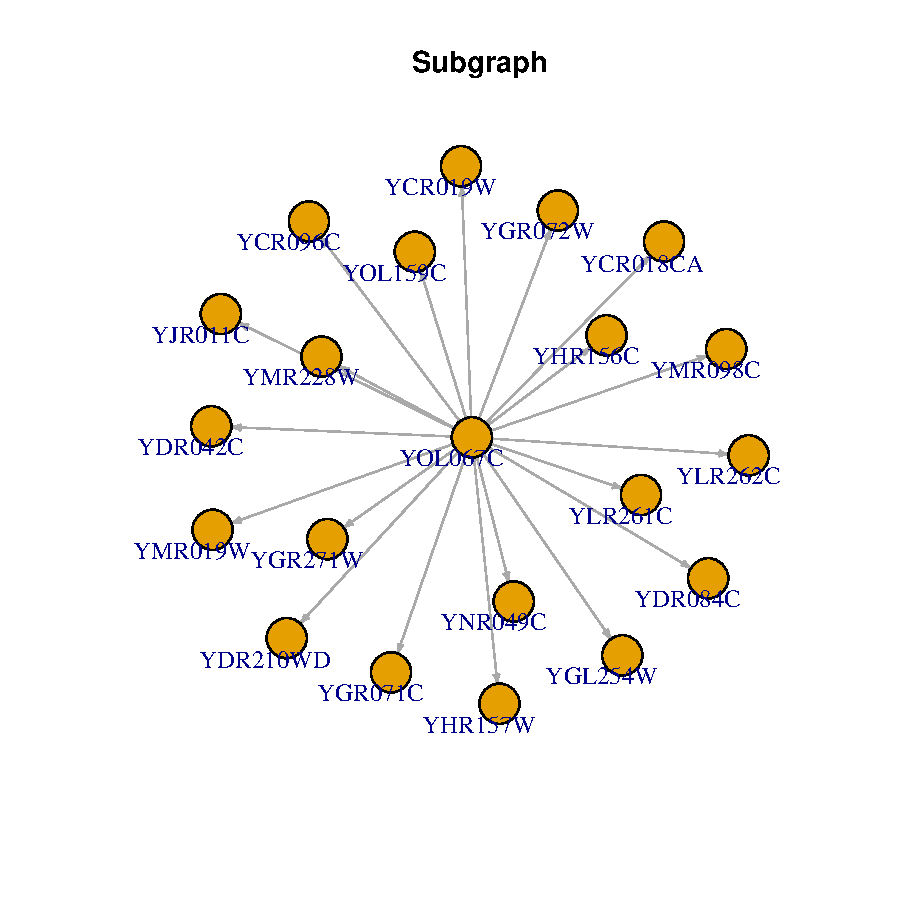
\includegraphics{graph-11c}

\begin{enumerate}
\item Let's use degree and authrity score as the two metrics. We find that node 'YOL067C' has biggest gap of the two metrics.
\item After plotting the subgraph, It's clear why this happen: this node has 20 out degrees and 0 in degree. So although it has big degree, it has low authority score, which is 0.
\end{enumerate}

\newpage
\question{2}{Running time}
\part{a}
\begin{Schunk}
\begin{Sinput}
> node.count = seq(from = 2000, to = 3000, by = 100)
> time.pr = rep(0, length(node.count))
> time.hits = rep(0, length(node.count))
> for (i in 1:length(node.count)){
+     n = node.count[i]
+     g <- sample_gnp(n, 1 / 20, directed = TRUE)
+     time.pr[i] = system.time(page.rank(g))
+     m = as.matrix(get.adjacency(g))
+     time.hits[i] = system.time(hits(m, 2))
+ }
> time.pr
\end{Sinput}
\begin{Soutput}
 [1] 0.017 0.026 0.021 0.023 0.026 0.027 0.029 0.033 0.035 0.037 0.039
\end{Soutput}
\begin{Sinput}
> time.hits
\end{Sinput}
\begin{Soutput}
 [1] 0.159 0.114 0.125 0.139 0.164 0.164 0.189 0.211 0.213 0.267 0.267
\end{Soutput}
\begin{Sinput}
> time.pr = time.pr / sum(time.pr)
> time.hits = time.hits / sum(time.hits)
> plot(node.count, time.pr, col = 'red', type = 'l')
> lines(node.count, time.hits, col = 'green', type = 'l')
\end{Sinput}
\end{Schunk}
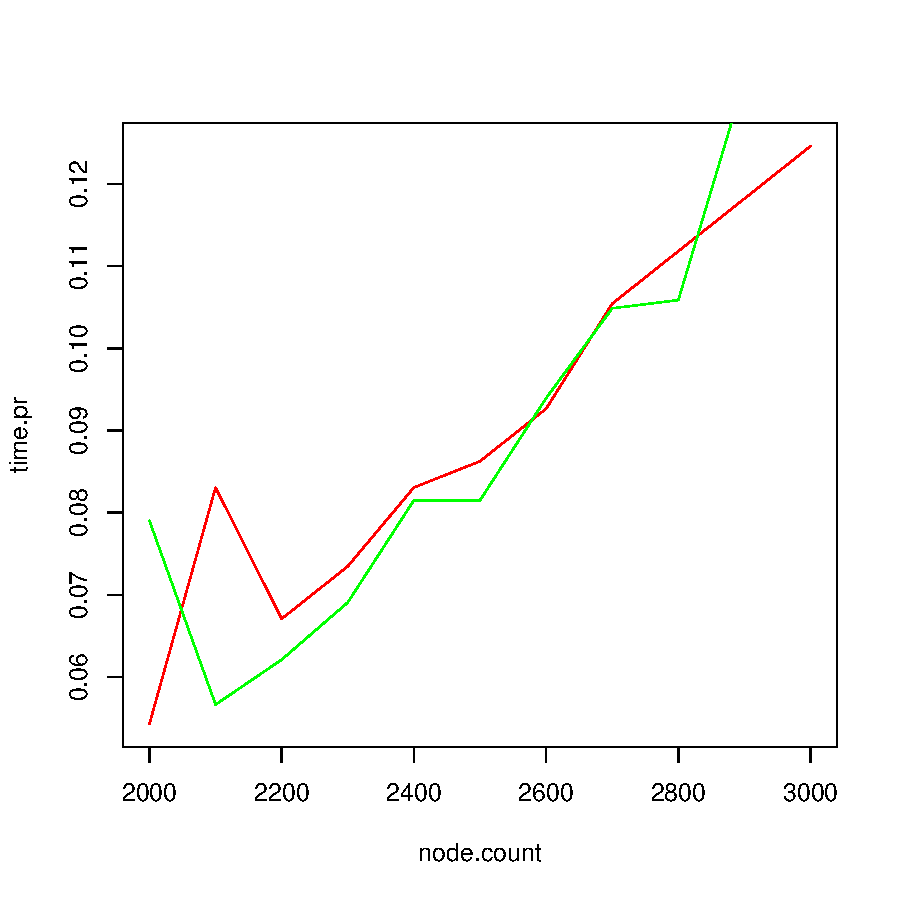
\includegraphics{graph-2a}

\part{b}
\begin{Schunk}
\begin{Sinput}
> for (i in 1:length(node.count)){
+     n = node.count[i]
+     g <- sample_gnp(n, 1 / 3, directed = TRUE)
+     time.pr[i] = system.time(page.rank(g))
+     m = as.matrix(get.adjacency(g))
+     time.hits[i] = system.time(hits(m, 3))
+ }
> time.pr
\end{Sinput}
\begin{Soutput}
 [1] 0.121 0.130 0.143 0.158 0.181 0.185 0.200 0.224 0.230 0.258 0.268
\end{Soutput}
\begin{Sinput}
> time.hits
\end{Sinput}
\begin{Soutput}
 [1] 0.158 0.171 0.186 0.206 0.239 0.245 0.290 0.326 0.339 0.379 0.423
\end{Soutput}
\begin{Sinput}
> time.pr = time.pr / sum(time.pr)
> time.hits = time.hits / sum(time.hits)
> plot(node.count, time.pr, col = 'red', type = 'l')
> lines(node.count, time.hits, col = 'green', type = 'l')
\end{Sinput}
\end{Schunk}
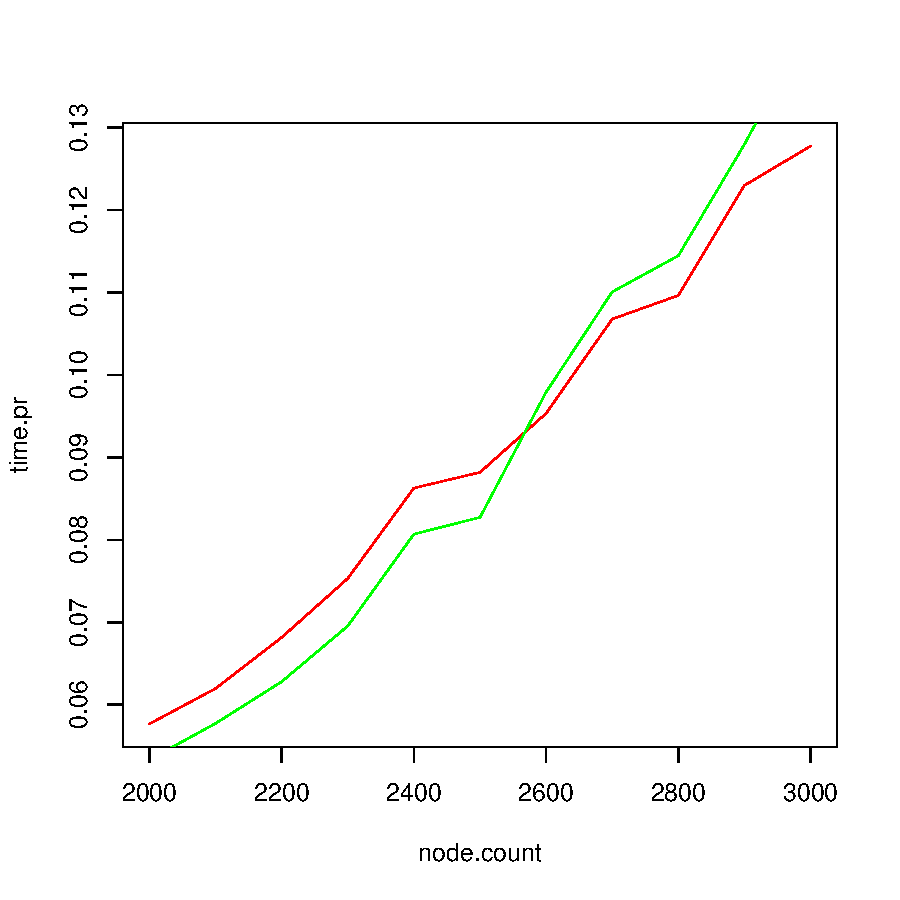
\includegraphics{graph-2b}

\begin{enumerate}
\item More nodes results in a increase in time to compute both PageRank and HITS.
\item Higher density result in a increase in time to compute both PageRank and HITS.
\item HITS needs more time than PageRank, which is 10 times, since it needs operation on matrix.
\item I have to scale them inorder to present in the same plot.
\end{enumerate}

\end{document}
